% Created 2018-10-09 Tue 20:33
% Intended LaTeX compiler: pdflatex
\documentclass[presentation]{beamer}
\usepackage[utf8]{inputenc}
\usepackage[T1]{fontenc}
\usepackage{graphicx}
\usepackage{grffile}
\usepackage{longtable}
\usepackage{wrapfig}
\usepackage{rotating}
\usepackage[normalem]{ulem}
\usepackage{amsmath}
\usepackage{textcomp}
\usepackage{amssymb}
\usepackage{capt-of}
\usepackage{natbib}
\usepackage[linktocpage,pdfstartview=FitH,colorlinks,
linkcolor=blue,anchorcolor=blue,
citecolor=blue,filecolor=blue,menucolor=blue,urlcolor=blue]{hyperref}
\setbeamertemplate{frame footer}{\insertshortauthor}
\setbeamerfont{page number in head/foot}{size=\tiny}
\setbeamercolor{footline}{fg=gray}
\author{Florian Hollenbach}
\usepackage[english]{isodate}
\usepackage{amsmath,amsthm,amssymb,amsfonts}
\usetheme{metropolis}
\usecolortheme{}
\usefonttheme{}
\useinnertheme{}
\useoutertheme{}
\author{Florian Hollenbach}
\date{\today}
\title{Political Science 209 - Fall 2018}
\subtitle{Linear Regression}

\hypersetup{
 pdfauthor={Florian Hollenbach},
 pdftitle={Political Science 209 - Fall 2018},
 pdfkeywords={},
 pdfsubject={},
 pdfcreator={Emacs 25.3.1 (Org mode 9.1.14)}, 
 pdflang={English}}
\begin{document}

\maketitle



\begin{frame}[label={sec:org95eb98e}]{Recall Correlation \& Scatterplot}
\begin{center}
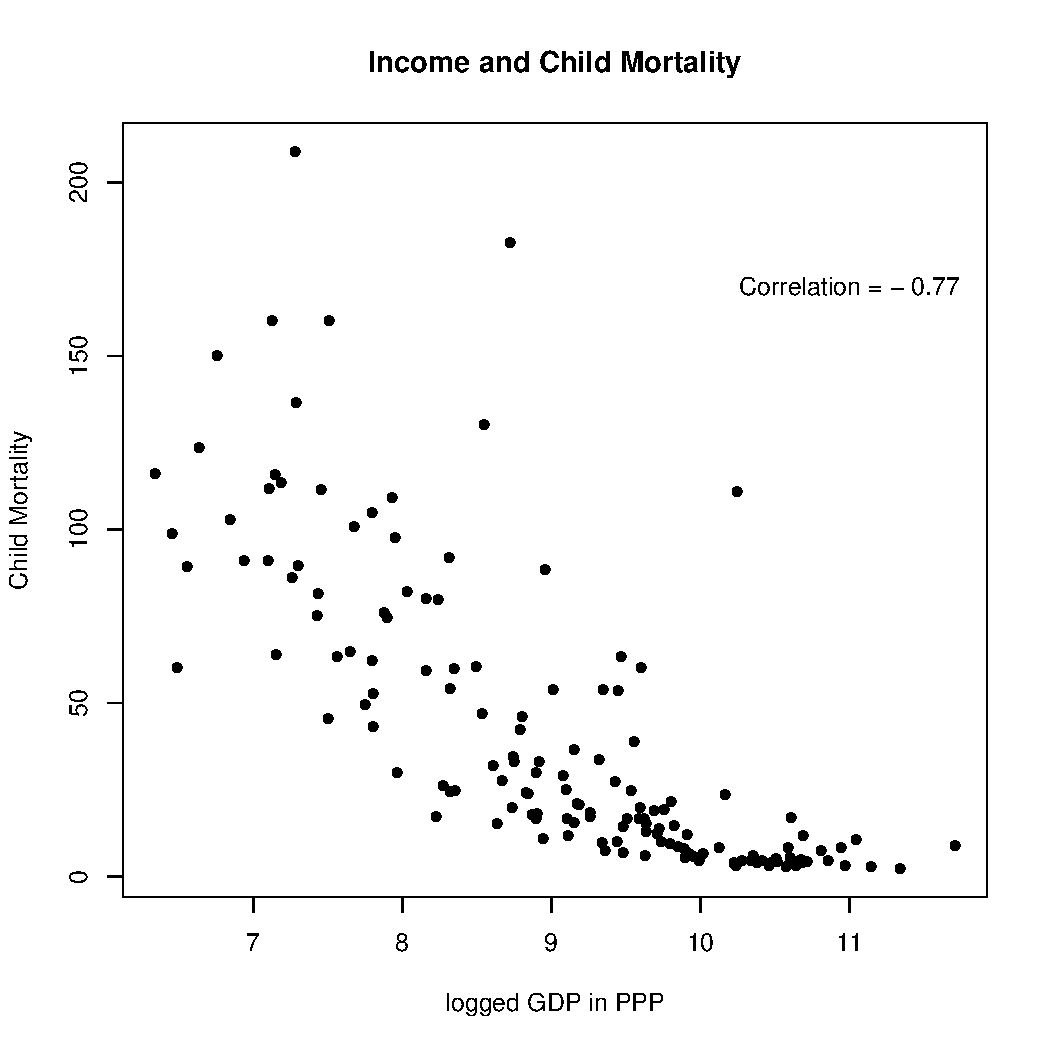
\includegraphics[width=6cm]{/Users/florianhollenbach/Documents/GitHub/Polisci209_2018/slides/week7/scatter_cor.pdf}
\end{center}

\alert{What is the correlation?}
\end{frame}

\begin{frame}[label={sec:org2f86292}]{Recall the definition of correlation}
Correlation (x,y) \(= \frac{1}{N} \sum^{N}_{i=1}\) z-score of \(x_i \times\) z-score of \(y_{i}\)

Correlation (x,y) \(= \frac{1}{N} \sum^{N}_{i=1} \frac{x_{i} - \bar{x}}{sd_{x}} \times   \frac{y_{i} - \bar{y}}{sd_{y}}\)
\end{frame}


\begin{frame}[label={sec:org55ce840}]{Correlations \& Scatterplots/Data points}
\begin{enumerate}
\item positive correlation \(\rightsquigarrow\) upward slope
\item negative correlation \(\rightsquigarrow\) downward slope
\item high correlation \(\rightsquigarrow\) tighter, close to a line
\item correlation \alert{cannot} capture nonlinear relationship
\end{enumerate}
\end{frame}

\begin{frame}[label={sec:orgff76387}]{Correlations \& Scatterplots/Data points}
\begin{center}
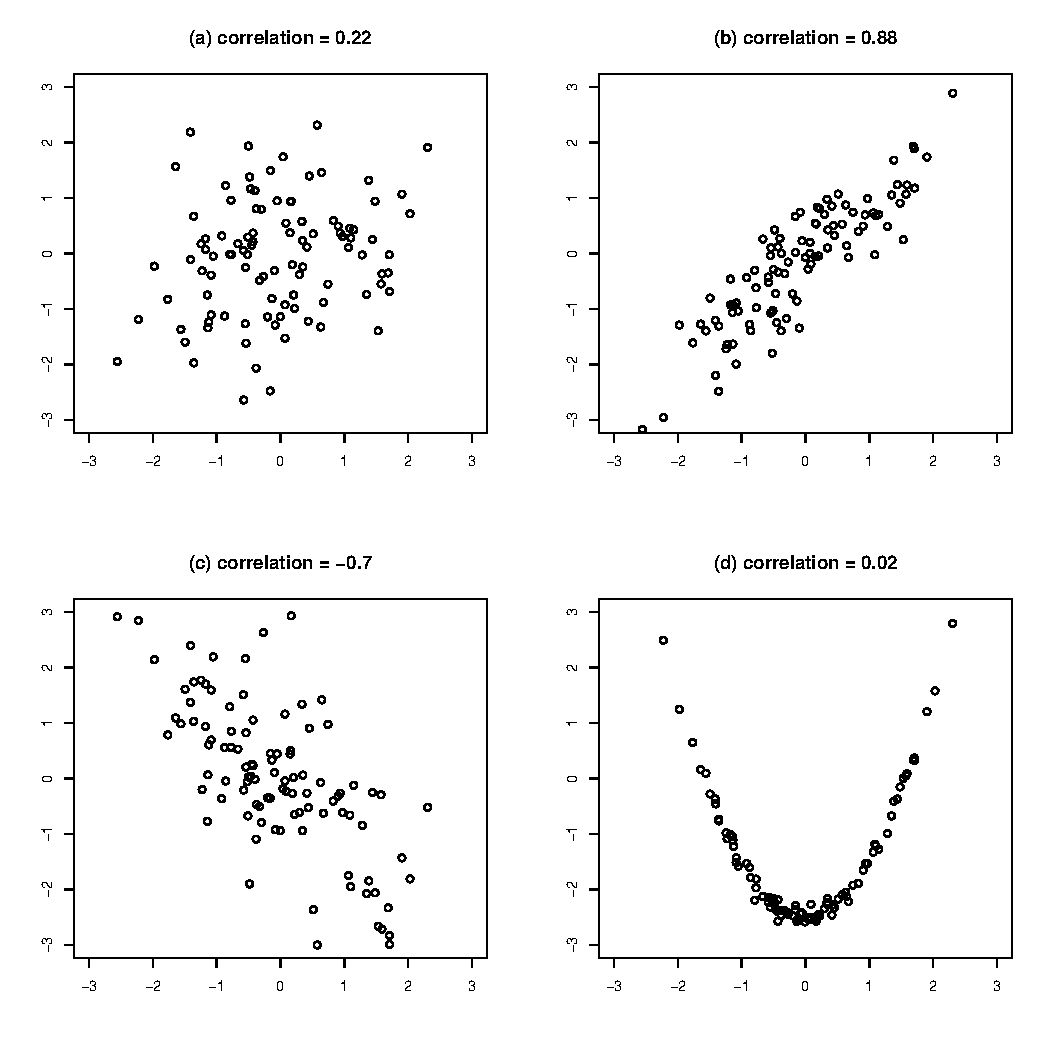
\includegraphics[width=8cm]{/Users/florianhollenbach/Documents/GitHub/Polisci209_2018/slides/week7/correlations.pdf}
\end{center}
\end{frame}


\begin{frame}[label={sec:orgea1585f}]{Moving from Correlation to Linear Regression}
Preview:
\begin{itemize}
\item linear regression allows us to create predictions
\item linear regression specifies direction of relationship
\item linear regression allows us to examine more than two variables at the same time (\emph{statistical control})
\end{itemize}
\end{frame}

\begin{frame}[label={sec:org3716a9a}]{Linear Regression}
\begin{itemize}
\item regression has one \alert{dependent (y)} and \emph{for now} one \alert{independent (x)} variable
\item regression is a statistical method to estimate the linear relationship between variables
\end{itemize}
\end{frame}

\begin{frame}[label={sec:org759736d}]{Linear Regression}
\begin{itemize}
\item goal of regression is to approximate the (linear) relationship between X and Y as best as possible
\end{itemize}
\pause
\begin{itemize}
\item regression is the mathematical model to draw best fitting line through cloud of points
\end{itemize}
\end{frame}


\begin{frame}[label={sec:org93ffc9c}]{Linear Regression}
\begin{center}
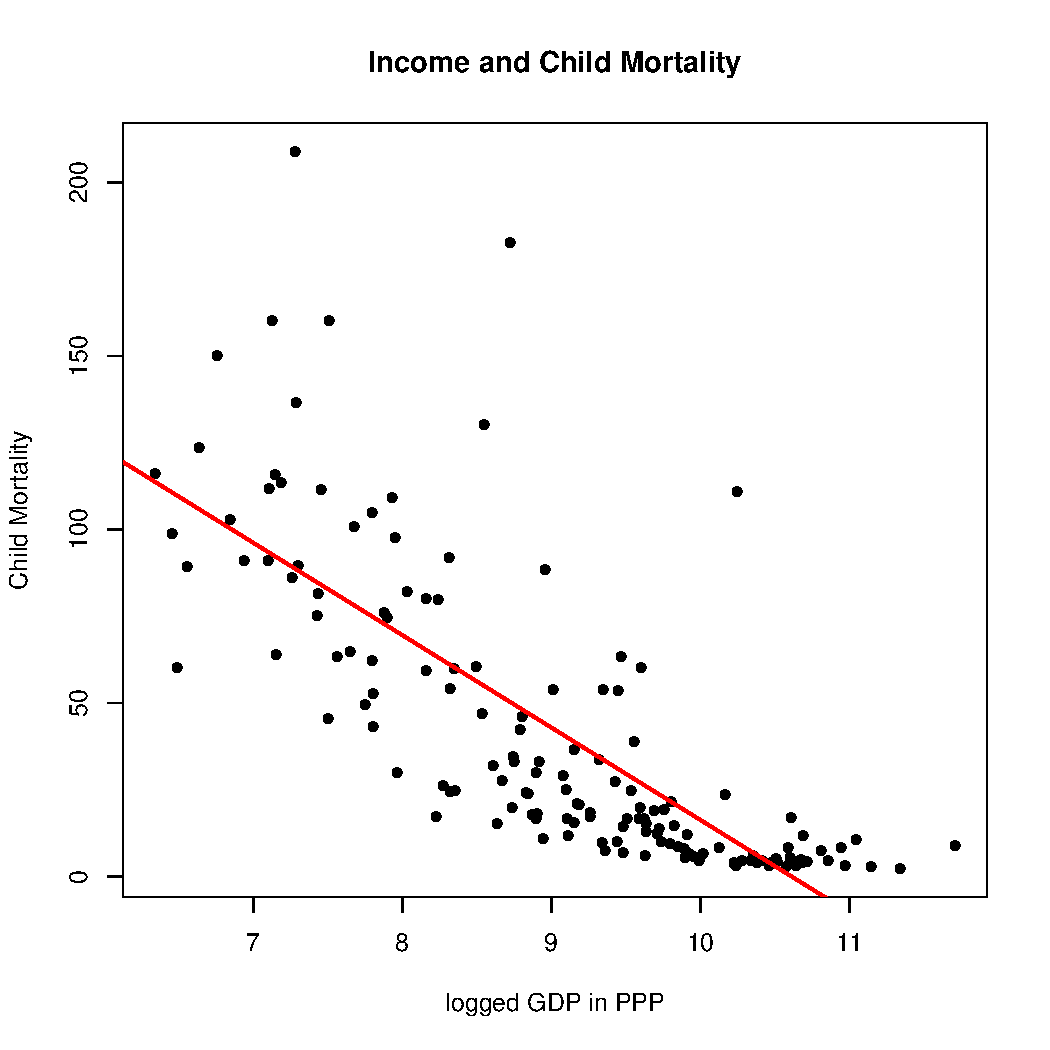
\includegraphics[width=5cm]{/Users/florianhollenbach/Documents/GitHub/Polisci209_2018/slides/week7/scatter_lm.pdf}
\end{center}

\alert{Linear regression is the mathematical model to draw best fitting line through cloud of points}
\end{frame}



\begin{frame}[label={sec:org43125e5}]{Linear Regression}
\begin{center}
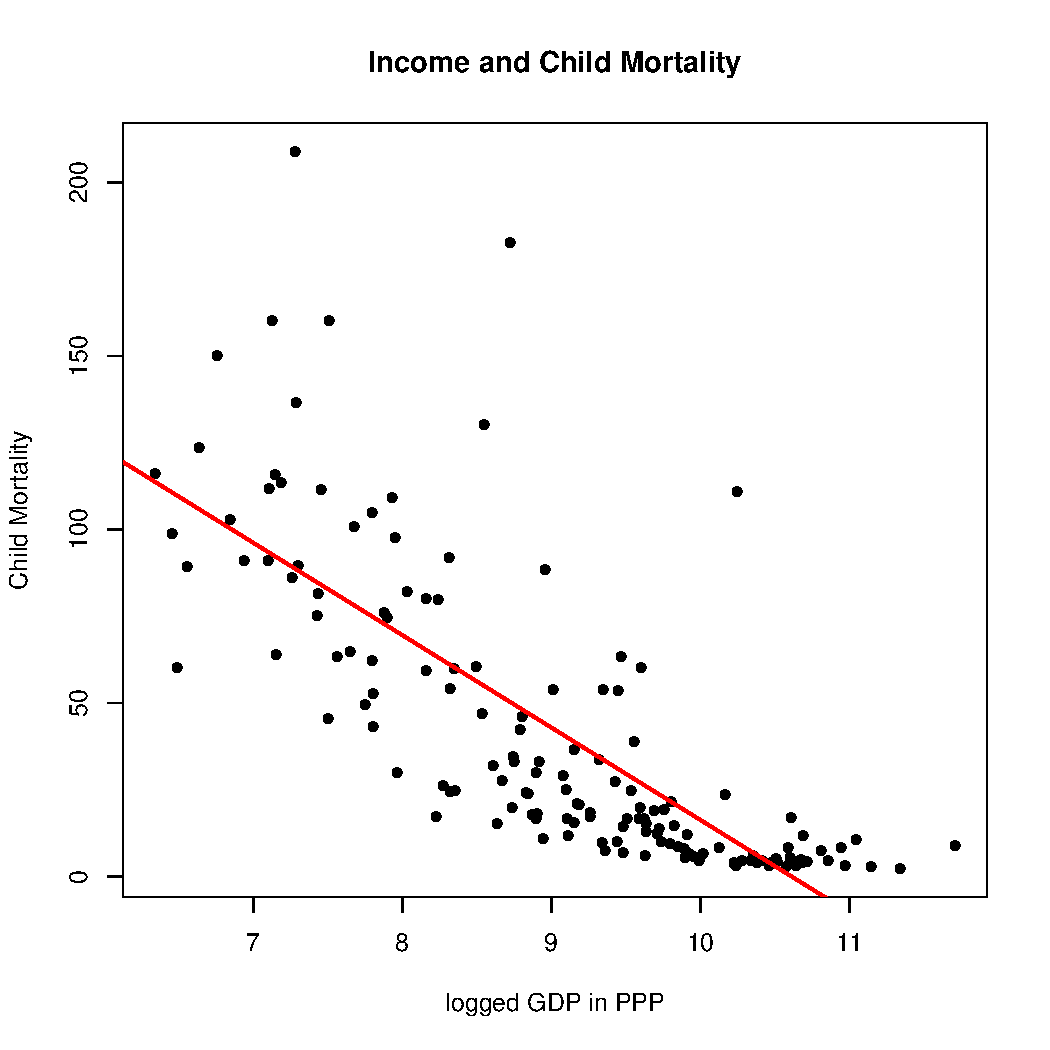
\includegraphics[width=4cm]{/Users/florianhollenbach/Documents/GitHub/Polisci209_2018/slides/week7/scatter_lm.pdf}
\end{center}

\begin{itemize}
\item regression line is an estimate of the (for now bivariate) relationship between x and y
\item for each x we have a prediction of y: \alert{what would we expect y to be given the value of x?}
\end{itemize}
\end{frame}


\begin{frame}[label={sec:org8f8cf1f}]{What is the equation of a line?}
\alert{Equation of a line?}
\pause
\(y = m  x + b\)

\(\rightarrow\) b? m?
\end{frame}


\begin{frame}[label={sec:org8756561}]{What is the equation of a line?}
\alert{Equation of a line?}

\(y = m  x + b\)

b \(\rightarrow\) y-intercept

m \(\rightarrow\) slope

\pause

\alert{regression equation:}

\(Y = \alpha + \beta  X + \epsilon\)

\(\rightarrow\) \(\alpha\)? \(\beta\)? \(\epsilon\)?
\end{frame}


\begin{frame}[label={sec:org36f4355}]{What is the equation of a line?}
\alert{Equation of a line?}

\(y = m  x + b\)

b \(\rightarrow\) y-intercept

m \(\rightarrow\) slope


\alert{regression equation:}

\(Y = alpha + \beta  X + \epsilon\)

\(\alpha\) \(\rightarrow\) y-intercept

\(\beta\) \(\rightarrow\) slope

\(\epsilon\) \(\rightarrow\) error
\end{frame}


\begin{frame}[label={sec:org0628870}]{Regression equation}
\begin{center}
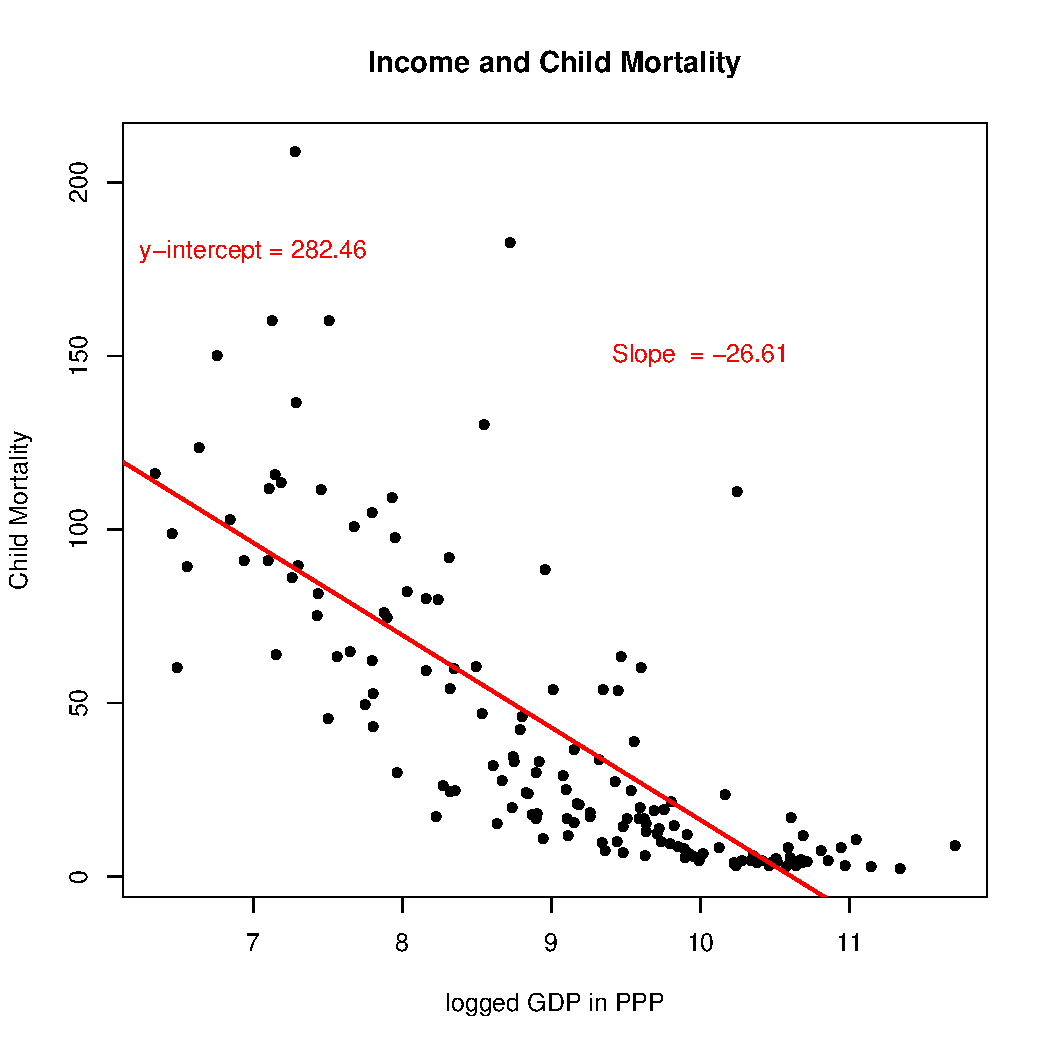
\includegraphics[width=7cm]{/Users/florianhollenbach/Documents/GitHub/Polisci209_2018/slides/week7/scatter_lm_text.pdf}
\end{center}
\end{frame}



\begin{frame}[label={sec:org890aa5f}]{Regression equation}
\begin{center}
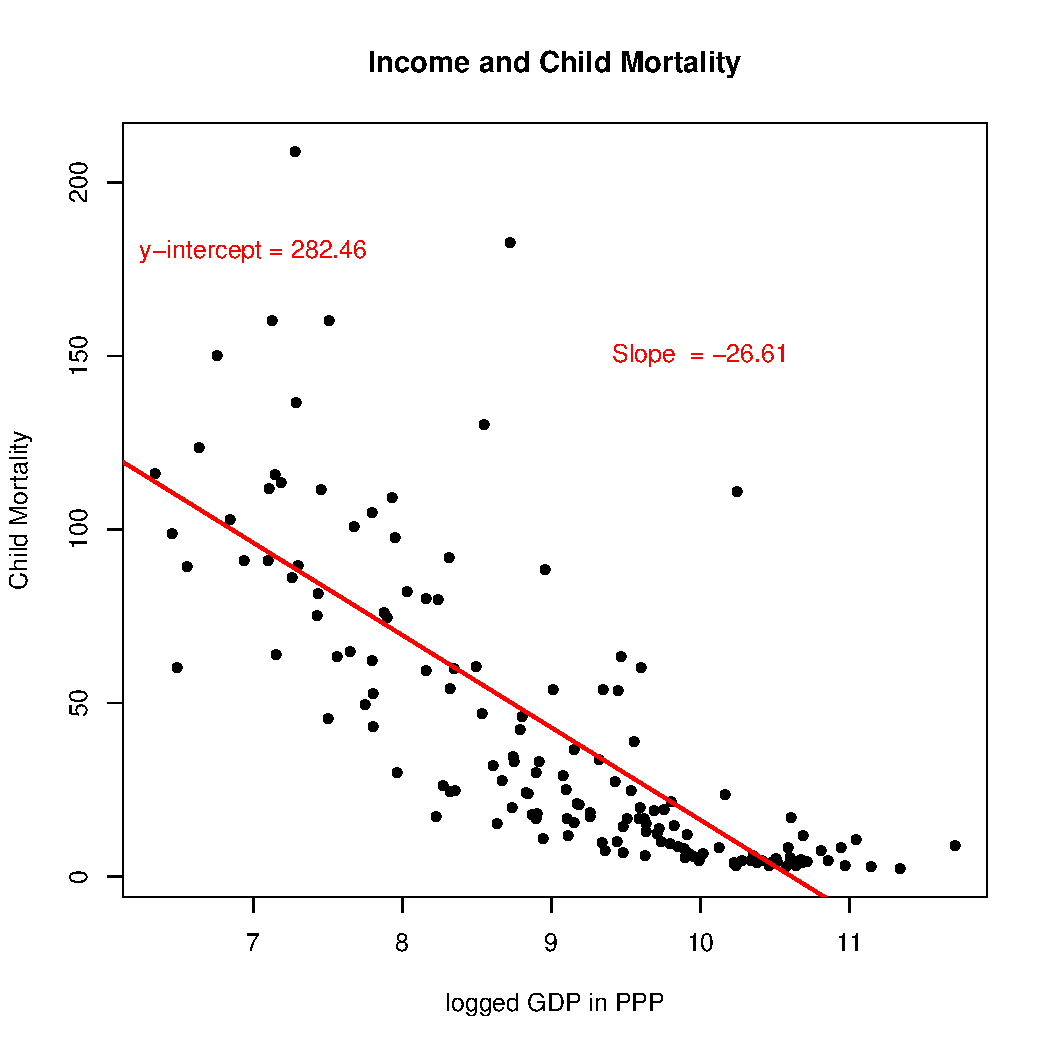
\includegraphics[width=5cm]{/Users/florianhollenbach/Documents/GitHub/Polisci209_2018/slides/week7/scatter_lm_text.pdf}
\end{center}

\(Y = 282.46 + -26.61  X + \epsilon\)
\end{frame}


\begin{frame}[label={sec:orgcd77a35}]{Regression equation}
\begin{itemize}
\item but, we don't know the equation that generates the data
\item our regression line is an estimate, based on the collected data
\end{itemize}

\pause

\begin{itemize}
\item estimates are denoted with little hats: \(\hat{\beta}\) and \(\hat{\alpha}\)
\end{itemize}

\pause

\begin{itemize}
\item \(\epsilon\) is an estimate of how good/bad our approximation is
\end{itemize}
\end{frame}
\end{document}